\documentclass[aspectratio=169,11pt]{beamer}
\usepackage[utf8]{inputenc}
\usepackage{xcolor}
\usepackage{setspace}
\usepackage{tabularx}
\usepackage{tikz}
\usepackage{pgfplots}
\pgfplotsset{compat=1.18}

% --- Typography ---
\usepackage[scaled=0.92]{helvet}
\renewcommand{\familydefault}{\sfdefault}

% --- Brand Palette ---
\definecolor{SolidBlack}{HTML}{000000}
\definecolor{PureWhite}{HTML}{FFFFFF}
\definecolor{LinkBlue}{HTML}{0066CC}
\definecolor{CorporateNavy}{HTML}{0A192F}
\definecolor{DeepCharcoal}{HTML}{2D3748}
\definecolor{RuleNavy}{HTML}{1E293B}

\setbeamercolor{background canvas}{bg=PureWhite}
\setbeamercolor{normal text}{fg=DeepCharcoal}
\setbeamertemplate{navigation symbols}{}

\begin{document}

% ==========================================
% SLIDE 1: COVER (unchanged)
% ==========================================
\begin{frame}
\vfill
\begin{tabularx}{\textwidth}{@{} X >{\raggedleft\arraybackslash}X @{}}
    {\fontsize{42}{48}\sffamily\bfseries\color{CorporateNavy} Muncheez\color{LinkBlue}{\textbf{.}}} & 
    \textsf{\small\bfseries\color{CorporateNavy} INVESTOR PRESENTATION} \\
    {\textsf{\scriptsize\bfseries\color{DeepCharcoal} THE NEIGHBORHOOD OPERATING SYSTEM}} & 
    \textsf{\scriptsize\color{LinkBlue}\bfseries PRE-SEED ROUND // 2026} \\
\end{tabularx}

\vspace{0.4cm}

\begin{tikzpicture}
    \draw[line width=2.5pt, color=CorporateNavy] (0,0) -- (\textwidth-3cm, 0);
    \draw[line width=2.5pt, color=LinkBlue] (\textwidth-3cm,0) -- (\textwidth, 0);
\end{tikzpicture}

\vspace{1.2cm}
{\fontsize{24}{30}\sffamily\bfseries\color{CorporateNavy} Convenience without compromise. Access without friction.}

\vspace{0.4cm}
\textsf{\small\color{DeepCharcoal} Starting in Thika Greens \textperiodcentered\ Ngoingwa \textperiodcentered\ Juja}

\vfill
\textsf{\tiny\bfseries\color{DeepCharcoal} CONFIDENTIAL // FOR QUALIFIED INVESTORS ONLY}
\end{frame}

% ==========================================
% SLIDE 2: THESIS (unchanged)
% ==========================================
\begin{frame}
\textsf{\scriptsize\bfseries\color{LinkBlue}\uppercase{01 / The Thesis}}
\vspace{0.2cm}

{\fontsize{22}{28}\sffamily\bfseries\color{CorporateNavy} The Access Problem}

\vspace{0.8cm}
\begin{tabularx}{\textwidth}{@{} X @{}}
    \textsf{\small \textperiodcentered\ Kenya has independent kitchens, bakers, cafés, home businesses.} \\
    \textsf{\small \textperiodcentered\ Discovery, ordering, payment, delivery are fragmented.} \\
    \textsf{\small \textperiodcentered\ Muncheez builds the missing infrastructure: Discover $\rightarrow$ Order $\rightarrow$ Pay $\rightarrow$ Fulfil $\rightarrow$ Deliver $\rightarrow$ Repeat.} \\
    \textsf{\small \textperiodcentered\ Start with food, scale to neighborhood commerce.}
\end{tabularx}
\end{frame}

% ==========================================
% SLIDE 3: THE GAP (unchanged)
% ==========================================
\begin{frame}
\textsf{\scriptsize\bfseries\color{LinkBlue}\uppercase{02 / The Gap}}
\vspace{0.2cm}

{\fontsize{22}{28}\sffamily\bfseries\color{CorporateNavy} Marketplaces vs. Neighborhood Layer}

\vspace{0.8cm}
\begin{tabularx}{\textwidth}{@{} X X @{}}
    \textsf{\small\bfseries\color{CorporateNavy} Current Marketplaces} & \textsf{\small\bfseries\color{CorporateNavy} Muncheez} \\
    \textsf{\small More listings = noise} & \textsf{\small Curated quality} \\
    \textsf{\small Best marketing wins} & \textsf{\small Best product wins} \\
    \textsf{\small Optimized for scale} & \textsf{\small Optimized for density} \\
    \textsf{\small Broad} & \textsf{\small Local}
\end{tabularx}
\vspace{0.4cm}
\textsf{\small We don't need 10k merchants – we need the \textit{right} 50–150 per neighborhood.}
\end{frame}

% ==========================================
% SLIDE 4: REDESIGNED – no diagram, pure table
% ==========================================
\begin{frame}
\textsf{\scriptsize\bfseries\color{LinkBlue}\uppercase{03 / Our Advantage}}
\vspace{0.2cm}

{\fontsize{22}{28}\sffamily\bfseries\color{CorporateNavy} Built for Neighborhood Density}

\vspace{0.8cm}
\begin{tabularx}{\textwidth}{@{} X @{}}
    \textsf{\small \textperiodcentered\ \textbf{Curated supply} – only the best local merchants, vetted by real reorder data.} \\
    \textsf{\small \textperiodcentered\ \textbf{Hyper‑local logistics} – routing optimized for unmapped streets and real‑time conditions.} \\
    \textsf{\small \textperiodcentered\ \textbf{Merchant‑first economics} – lower commissions (12–15\% vs. 30\%) and instant M‑PESA payouts.} \\
    \textsf{\small \textperiodcentered\ \textbf{Community trust} – we become the neighborhood's go‑to for reliable delivery.}
\end{tabularx}
\vspace{0.4cm}
\textsf{\small Not a smaller Glovo – a smarter, more local operating system.}
\end{frame}

% ==========================================
% SLIDE 5: REDESIGNED – no diagram, just table
% ==========================================
\begin{frame}
\textsf{\scriptsize\bfseries\color{LinkBlue}\uppercase{04 / Convenience + Access}}
\vspace{0.2cm}

{\fontsize{22}{28}\sffamily\bfseries\color{CorporateNavy} One Ecosystem for All}

\vspace{0.8cm}
\begin{tabularx}{\textwidth}{@{} X X X @{}}
    \textsf{\small\bfseries\color{CorporateNavy} Customers} & \textsf{\small\bfseries\color{CorporateNavy} Merchants} & \textsf{\small\bfseries\color{CorporateNavy} Riders} \\
    \textsf{\small Discover, order, pay, track, receive} & \textsf{\small List, manage, fulfil, get paid daily} & \textsf{\small Matched routes, higher earnings}
\end{tabularx}
\vspace{0.4cm}
\textsf{\small One platform, three simple experiences.}
\end{frame}

% ==========================================
% SLIDE 6: THE ECOSYSTEM (unchanged)
% ==========================================
\begin{frame}
\textsf{\scriptsize\bfseries\color{LinkBlue}\uppercase{05 / The Ecosystem}}
\vspace{0.2cm}

{\fontsize{22}{28}\sffamily\bfseries\color{CorporateNavy} Three-Sided Network}

\vspace{0.8cm}
\begin{tabularx}{\textwidth}{@{} X X X @{}}
    \textsf{\small\bfseries\color{CorporateNavy} Customers} & \textsf{\small\bfseries\color{CorporateNavy} Merchants} & \textsf{\small\bfseries\color{CorporateNavy} Riders} \\
    \textsf{\small Discover} & \textsf{\small List} & \textsf{\small Get matched} \\
    \textsf{\small Order} & \textsf{\small Sell} & \textsf{\small Pick up} \\
    \textsf{\small Pay} & \textsf{\small Manage} & \textsf{\small Deliver} \\
    \textsf{\small Track} & \textsf{\small Fulfil} & \textsf{\small Earn} \\
    \textsf{\small Receive} & \textsf{\small Get paid} & 
\end{tabularx}
\vspace{0.4cm}
\textsf{\small One platform orchestrates every step.}
\end{frame}

% ==========================================
% SLIDE 7: DENSITY FIRST (unchanged)
% ==========================================
\begin{frame}
\textsf{\scriptsize\bfseries\color{LinkBlue}\uppercase{06 / Density First}}
\vspace{0.2cm}

{\fontsize{22}{28}\sffamily\bfseries\color{CorporateNavy} Win Neighborhoods, Not Cities}

\vspace{0.8cm}
\begin{tabularx}{\textwidth}{@{} X @{}}
    \textsf{\small \textperiodcentered\ Launch in Thika Greens, Ngoingwa, Juja.} \\
    \textsf{\small \textperiodcentered\ Juja: 300k population (2019) – educational hub.} \\
    \textsf{\small \textperiodcentered\ Thika: 279k population – commercial hub.} \\
    \textsf{\small \textperiodcentered\ Strategy: win 3 neighborhoods before 10 towns.}
\end{tabularx}
\end{frame}

% ==========================================
% SLIDE 8: CURATED MERCHANTS (unchanged)
% ==========================================
\begin{frame}
\textsf{\scriptsize\bfseries\color{LinkBlue}\uppercase{07 / Curated Network}}
\vspace{0.2cm}

{\fontsize{22}{28}\sffamily\bfseries\color{CorporateNavy} Onboard the Best, Not the Most}

\vspace{0.8cm}
\begin{tabularx}{\textwidth}{@{} X X X @{}}
    \textsf{\small Restaurants} & \textsf{\small Home Kitchens} & \textsf{\small Bakers} \\
    \textsf{\small Kuku choma} & \textsf{\small Swahili food} & \textsf{\small Sourdough} \\
    \textsf{\small Nyama choma} & \textsf{\small Healthy food} & \textsf{\small Pastries} \\
    \textsf{\small African cuisine} & \textsf{\small Desserts} & \textsf{\small Cakes} \\
    \textsf{\small Cafés} & \textsf{\small Student-focused} & \textsf{\small Hidden gems}
\end{tabularx}
\vspace{0.4cm}
\textsf{\small Products people actively seek.}
\end{frame}

% ==========================================
% SLIDE 9: CURATION ENGINE (unchanged)
% ==========================================
\begin{frame}
\textsf{\scriptsize\bfseries\color{LinkBlue}\uppercase{08 / The Curation Engine}}
\vspace{0.2cm}

{\fontsize{22}{28}\sffamily\bfseries\color{CorporateNavy} Measure What Reorders}

\vspace{0.8cm}
\begin{tabularx}{\textwidth}{@{} X X @{}}
    \textsf{\small\bfseries\color{CorporateNavy} Product Quality} & \textsf{\small taste, consistency, portion, presentation} \\
    \textsf{\small\bfseries\color{CorporateNavy} Operational Quality} & \textsf{\small prep time, accuracy, packaging} \\
    \textsf{\small\bfseries\color{CorporateNavy} Customer Quality} & \textsf{\small rating, repeat, refund rate} \\
    \textsf{\small\bfseries\color{CorporateNavy} Commercial Quality} & \textsf{\small AOV, conversion, demand}
\end{tabularx}
\vspace{0.4cm}
\textsf{\small Learn: what people \textit{say} vs what they \textit{reorder}.}
\end{frame}

% ==========================================
% SLIDE 10: LOGISTICS CHALLENGE (unchanged)
% ==========================================
\begin{frame}
\textsf{\scriptsize\bfseries\color{LinkBlue}\uppercase{09 / The Logistics Challenge}}
\vspace{0.2cm}

{\fontsize{22}{28}\sffamily\bfseries\color{CorporateNavy} Nairobi's Streets Are Not a Grid}

\vspace{0.8cm}
\begin{tabularx}{\textwidth}{@{} X @{}}
    \textsf{\small \textperiodcentered\ Slow restaurants} \\
    \textsf{\small \textperiodcentered\ Rider distance} \\
    \textsf{\small \textperiodcentered\ Traffic} \\
    \textsf{\small \textperiodcentered\ Ambiguous addresses} \\
    \textsf{\small \textperiodcentered\ Unavailable customers} \\
    \textsf{\small \textperiodcentered\ Inaccessible roads} \\
    \textsf{\small \textperiodcentered\ Food ready / not ready mismatch}
\end{tabularx}
\vspace{0.2cm}
\textsf{\small Shortest‑path routing is not enough.}
\end{frame}

% ==========================================
% SLIDE 11: LOGISTICS ENGINE (unchanged)
% ==========================================
\begin{frame}
\textsf{\scriptsize\bfseries\color{LinkBlue}\uppercase{10 / Our Logistics Engine}}
\vspace{0.2cm}

{\fontsize{22}{28}\sffamily\bfseries\color{CorporateNavy} Zone, Predict, Dispatch}

\vspace{0.8cm}
\begin{enumerate}
    \item \textbf{Zone:} Dynamic neighborhood zones (TG, NG, JJ).
    \item \textbf{Predict:} Learn each merchant's real prep time.
    \item \textbf{Score:} Combine distance, prep, workload, traffic, reliability.
    \item \textbf{Batch:} One rider, multiple deliveries, optimized route.
\end{enumerate}
\vspace{0.2cm}
\textsf{\small Goal: lowest‑risk successful delivery.}
\end{frame}

% ==========================================
% SLIDE 12: REDESIGNED – no diagram, pure text
% ==========================================
\begin{frame}
\textsf{\scriptsize\bfseries\color{LinkBlue}\uppercase{11 / Density Economics}}
\vspace{0.2cm}

{\fontsize{22}{28}\sffamily\bfseries\color{CorporateNavy} Why Density Wins}

\vspace{0.8cm}
\begin{tabularx}{\textwidth}{@{} X @{}}
    \textsf{\small \textperiodcentered\ \textbf{Better unit economics:} one rider can handle 2–3 deliveries per trip.} \\
    \textsf{\small \textperiodcentered\ \textbf{Faster delivery:} shorter travel distances, fewer delays.} \\
    \textsf{\small \textperiodcentered\ \textbf{Higher rider earnings:} more orders per hour, better retention.} \\
    \textsf{\small \textperiodcentered\ \textbf{Stronger network effects:} each new user makes the system more valuable.}
\end{tabularx}
\vspace{0.4cm}
\textsf{\small We build density before geography – it's our structural advantage.}
\end{frame}

% ==========================================
% SLIDE 13: DATA FLYWHEEL (unchanged – keep diagram, it's standard)
% ==========================================
\begin{frame}
\textsf{\scriptsize\bfseries\color{LinkBlue}\uppercase{12 / The Data Flywheel}}
\vspace{0.2cm}

{\fontsize{22}{28}\sffamily\bfseries\color{CorporateNavy} Every Order Makes Us Smarter}

\vspace{0.8cm}
\centering
\begin{tikzpicture}[node distance=0.8cm, auto]
  \node (o) [draw, rectangle, fill=LinkBlue!10, text=CorporateNavy, minimum width=2.8cm] {Order};
  \node (m) [draw, rectangle, fill=LinkBlue!10, text=CorporateNavy, below=of o] {Merchant prep};
  \node (r) [draw, rectangle, fill=LinkBlue!10, text=CorporateNavy, below=of m] {Rider movement};
  \node (d) [draw, rectangle, fill=LinkBlue!10, text=CorporateNavy, below=of r] {Delivery time};
  \node (c) [draw, rectangle, fill=LinkBlue!10, text=CorporateNavy, below=of d] {Customer behavior};
  \node (p) [draw, rectangle, fill=LinkBlue!10, text=CorporateNavy, below=of c] {Demand patterns};
  \node (b) [draw, rectangle, fill=CorporateNavy!20, text=CorporateNavy, below=of p] {Better ranking, dispatch, ETA};
  \node (rep) [draw, rectangle, fill=CorporateNavy!20, text=CorporateNavy, below=of b] {Repeat orders \& density};
  \draw[->, thick] (o) -- (m);
  \draw[->, thick] (m) -- (r);
  \draw[->, thick] (r) -- (d);
  \draw[->, thick] (d) -- (c);
  \draw[->, thick] (c) -- (p);
  \draw[->, thick] (p) -- (b);
  \draw[->, thick] (b) -- (rep);
  \draw[->, thick, bend left] (rep.east) to [out=0,in=0] (o.east);
\end{tikzpicture}
\end{frame}

% ==========================================
% SLIDE 14: REDESIGNED – no diagram, simple table
% ==========================================
\begin{frame}
\textsf{\scriptsize\bfseries\color{LinkBlue}\uppercase{13 / Technology Roadmap}}
\vspace{0.2cm}

{\fontsize{22}{28}\sffamily\bfseries\color{CorporateNavy} From MVP to Ecosystem}

\vspace{0.8cm}
\begin{tabularx}{\textwidth}{@{} p{2.5cm} X @{}}
    \textsf{\small\bfseries\color{LinkBlue} Now (Phase 1)} & \textsf{\small Core transaction engine, merchant dashboard, rider app, M‑PESA integration.} \\[0.3cm]
    \textsf{\small\bfseries\color{LinkBlue} Q2 2026 (Phase 2)} & \textsf{\small Dispatch intelligence, ETA prediction, dynamic batching, merchant analytics.} \\[0.3cm]
    \textsf{\small\bfseries\color{LinkBlue} Q4 2026 (Phase 3)} & \textsf{\small Personalized discovery, demand forecasting, neighborhood growth tools.}
\end{tabularx}
\vspace{0.4cm}
\textsf{\small This pre‑seed powers Phase 1 & 2 – building the moat.}
\end{frame}

% ==========================================
% SLIDE 15: BEYOND FOOD (unchanged)
% ==========================================
\begin{frame}
\textsf{\scriptsize\bfseries\color{LinkBlue}\uppercase{14 / Beyond Food}}
\vspace{0.2cm}

{\fontsize{22}{28}\sffamily\bfseries\color{CorporateNavy} Entry → Neighborhood Commerce}

\vspace{0.8cm}
\begin{tabularx}{\textwidth}{@{} X X X @{}}
    \textsf{\small\bfseries\color{CorporateNavy} Today} & \textsf{\small\bfseries\color{CorporateNavy} Next} & \textsf{\small\bfseries\color{CorporateNavy} Later} \\
    \textsf{\small Food} & \textsf{\small Groceries} & \textsf{\small Laundry} \\
    & \textsf{\small Bakery} & \textsf{\small Local services} \\
    & \textsf{\small Specialty foods} & \textsf{\small Errands} \\
    & \textsf{\small Pharmacies} & \textsf{\small Neighborhood commerce} \\
    & \textsf{\small Flowers} & 
\end{tabularx}
\vspace{0.4cm}
\textsf{\small Infrastructure allows categories to plug in.}
\end{frame}

% ==========================================
% SLIDE 16: BUSINESS MODEL (unchanged)
% ==========================================
\begin{frame}
\textsf{\scriptsize\bfseries\color{LinkBlue}\uppercase{15 / Revenue Streams}}
\vspace{0.2cm}

{\fontsize{22}{28}\sffamily\bfseries\color{CorporateNavy} Monetize the Ecosystem}

\vspace{0.8cm}
\begin{tabularx}{\textwidth}{@{} X X @{}}
    \textsf{\small\bfseries\color{CorporateNavy} Merchant Commission} & \textsf{\small 12–15\% (below Glovo's 30\%)} \\
    \textsf{\small\bfseries\color{CorporateNavy} Delivery Margin} & \textsf{\small Customer fee – rider payout} \\
    \textsf{\small\bfseries\color{CorporateNavy} Merchant Tools} & \textsf{\small Analytics, promoted placement} \\
    \textsf{\small\bfseries\color{CorporateNavy} Membership} & \textsf{\small Subscription for reduced fees}
\end{tabularx}
\vspace{0.4cm}
\textsf{\small We make money when the ecosystem moves.}
\end{frame}

% ==========================================
% SLIDE 17: UNIT ECONOMICS (unchanged)
% ==========================================
\begin{frame}
\textsf{\scriptsize\bfseries\color{LinkBlue}\uppercase{16 / Unit Economics}}
\vspace{0.2cm}

{\fontsize{22}{28}\sffamily\bfseries\color{CorporateNavy} Contribution per Order}

\vspace{0.8cm}
\begin{tabularx}{\textwidth}{@{} X r @{}}
    \textsf{\small Average Order Value (AOV)} & \textsf{\small KES 900} \\
    \textsf{\small Commission (12\%)} & \textsf{\small KES 108} \\
    \textsf{\small Delivery Fee (customer)} & \textsf{\small KES 100} \\
    \textsf{\small Rider Payout} & \textsf{\small KES 90} \\
    \textsf{\small Payment Cost} & \textsf{\small KES 18} \\
    \hline
    \textsf{\small \textbf{Contribution}} & \textsf{\small \textbf{KES 100}}
\end{tabularx}
\vspace{0.4cm}
\textsf{\small Improves with density, batching, repeat customers.}
\end{frame}

% ==========================================
% SLIDE 18: ACQUISITION CHANNELS (unchanged)
% ==========================================
\begin{frame}
\textsf{\scriptsize\bfseries\color{LinkBlue}\uppercase{17 / Growth Channels}}
\vspace{0.2cm}

{\fontsize{22}{28}\sffamily\bfseries\color{CorporateNavy} Neighborhood Density, Not Mass Marketing}

\vspace{0.8cm}
\begin{tabularx}{\textwidth}{@{} X @{}}
    \textsf{\small \textperiodcentered\ Merchant-led: each brings existing customers} \\
    \textsf{\small \textperiodcentered\ Campus: Juja's student population} \\
    \textsf{\small \textperiodcentered\ Neighborhood ambassadors} \\
    \textsf{\small \textperiodcentered\ Referral loops} \\
    \textsf{\small \textperiodcentered\ Content: discover hidden gems} \\
    \textsf{\small \textperiodcentered\ WhatsApp: orders, offers, community} \\
    \textsf{\small \textperiodcentered\ Local partnerships: apartments, offices, gyms}
\end{tabularx}
\vspace{0.4cm}
\textsf{\small Our strongest asset: the merchants themselves.}
\end{frame}

% ==========================================
% SLIDE 19: REDESIGNED – no diagram, clean table
% ==========================================
\begin{frame}
\textsf{\scriptsize\bfseries\color{LinkBlue}\uppercase{18 / Growth Milestones}}
\vspace{0.2cm}

{\fontsize{22}{28}\sffamily\bfseries\color{CorporateNavy} 18‑Month Execution Plan}

\vspace{0.8cm}
\begin{tabularx}{\textwidth}{@{} p{2.2cm} X @{}}
    \textsf{\small\bfseries\color{LinkBlue} Months 0–6} & \textsf{\small Launch pilot: 50+ merchants, 1,000+ customers, 4k monthly orders.} \\
    \textsf{\small\bfseries\color{LinkBlue} Months 6–12} & \textsf{\small Scale density: 150+ merchants, 10k+ customers, 15k monthly orders.} \\
    \textsf{\small\bfseries\color{LinkBlue} Months 12–18} & \textsf{\small Expand to adjacent hubs, reach 30k monthly orders, KES 27M GMV.}
\end{tabularx}
\vspace{0.4cm}
\textsf{\small Each phase builds the data and network effect for the next.}
\end{frame}

% ==========================================
% SLIDE 20: REDESIGNED – chart is okay, but we keep it clean; no extra diagrams
% ==========================================
\begin{frame}
\textsf{\scriptsize\bfseries\color{LinkBlue}\uppercase{19 / Growth Trajectory}}
\vspace{0.2cm}

{\fontsize{22}{28}\sffamily\bfseries\color{CorporateNavy} Monthly Orders, Merchants, Riders}

\vspace{0.4cm}
\begin{tikzpicture}
\begin{axis}[
  xlabel=Month,
  ylabel=Orders / Merchants / Riders,
  xmin=0, xmax=18,
  ymin=0, ymax=35000,
  legend pos=north west,
  grid=major,
  width=0.9\textwidth, height=0.35\textheight,
  xtick={1,3,6,9,12,18},
  legend style={font=\small}
]
\addplot[color=LinkBlue, mark=*, thick] coordinates {
  (1,300) (3,1200) (6,4000) (9,8000) (12,15000) (18,30000)
};
\addlegendentry{Orders}
\addplot[color=CorporateNavy, mark=square, thick] coordinates {
  (1,15) (3,30) (6,50) (9,75) (12,110) (18,175)
};
\addlegendentry{Merchants}
\addplot[color=DeepCharcoal, mark=triangle, thick] coordinates {
  (1,8) (3,15) (6,25) (9,35) (12,50) (18,75)
};
\addlegendentry{Riders}
\end{axis}
\end{tikzpicture}
\vspace{0.2cm}
\begin{tabularx}{\textwidth}{@{} X r @{}}
    \textsf{\small At 30k monthly orders} & \textsf{\small KES 27M GMV} \\
    \textsf{\small With 175+ merchants} & \textsf{\small KES 3.2M monthly commission}
\end{tabularx}
\end{frame}

% ==========================================
% SLIDE 21: USE OF FUNDS (unchanged)
% ==========================================
\begin{frame}
\textsf{\scriptsize\bfseries\color{LinkBlue}\uppercase{20 / Use of Funds}}
\vspace{0.2cm}

{\fontsize{22}{28}\sffamily\bfseries\color{CorporateNavy} KES 3,000,000 Allocation}

\vspace{0.4cm}
\begin{center}
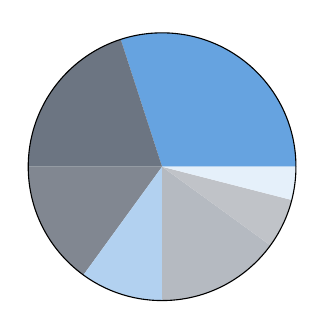
\begin{tikzpicture}[scale=0.85]
  \def\angleA{108}\def\angleB{72}\def\angleC{54}
  \def\angleD{36}\def\angleE{54}\def\angleF{21.6}\def\angleG{14.4}
  \fill[LinkBlue!60] (0,0) -- (0:2) arc (0:\angleA:2) -- cycle;
  \fill[CorporateNavy!60] (0,0) -- (\angleA:2) arc (\angleA:\angleA+\angleB:2) -- cycle;
  \fill[DeepCharcoal!60] (0,0) -- (\angleA+\angleB:2) arc (\angleA+\angleB:\angleA+\angleB+\angleC:2) -- cycle;
  \fill[LinkBlue!30] (0,0) -- (\angleA+\angleB+\angleC:2) arc (\angleA+\angleB+\angleC:\angleA+\angleB+\angleC+\angleD:2) -- cycle;
  \fill[CorporateNavy!30] (0,0) -- (\angleA+\angleB+\angleC+\angleD:2) arc (\angleA+\angleB+\angleC+\angleD:\angleA+\angleB+\angleC+\angleD+\angleE:2) -- cycle;
  \fill[DeepCharcoal!30] (0,0) -- (\angleA+\angleB+\angleC+\angleD+\angleE:2) arc (\angleA+\angleB+\angleC+\angleD+\angleE:\angleA+\angleB+\angleC+\angleD+\angleE+\angleF:2) -- cycle;
  \fill[LinkBlue!10] (0,0) -- (\angleA+\angleB+\angleC+\angleD+\angleE+\angleF:2) arc (\angleA+\angleB+\angleC+\angleD+\angleE+\angleF:360:2) -- cycle;
  \draw (0,0) circle (2);
\end{tikzpicture}
\end{center}
\vspace{0.2cm}
\begin{tabularx}{\textwidth}{@{} X r @{}}
    \textsf{\small Engineering \& Infrastructure} & \textsf{\small 30\% (KES 900k)} \\
    \textsf{\small Operations \& Logistics} & \textsf{\small 20\% (KES 600k)} \\
    \textsf{\small Growth} & \textsf{\small 15\% (KES 450k)} \\
    \textsf{\small Merchant Onboarding} & \textsf{\small 10\% (KES 300k)} \\
    \textsf{\small Working Capital} & \textsf{\small 15\% (KES 450k)} \\
    \textsf{\small Legal \& Admin} & \textsf{\small 6\% (KES 180k)} \\
    \textsf{\small Contingency} & \textsf{\small 4\% (KES 120k)}
\end{tabularx}
\end{frame}

% ==========================================
% SLIDE 22: ENGINEERING MOAT (unchanged)
% ==========================================
\begin{frame}
\textsf{\scriptsize\bfseries\color{LinkBlue}\uppercase{21 / Engineering is the Moat}}
\vspace{0.2cm}

{\fontsize{22}{28}\sffamily\bfseries\color{CorporateNavy} Build the Infrastructure}

\vspace{0.8cm}
\begin{tabularx}{\textwidth}{@{} X @{}}
    \textsf{\small \textperiodcentered\ Reliable transaction engine} \\
    \textsf{\small \textperiodcentered\ Fulfilment state machine (Placed→…→Delivered)} \\
    \textsf{\small \textperiodcentered\ Dispatch engine (right rider, right time)} \\
    \textsf{\small \textperiodcentered\ Data layer: every order improves the system} \\
    \textsf{\small \textperiodcentered\ Simple merchant tools} \\
    \textsf{\small \textperiodcentered\ M-PESA API integration}
\end{tabularx}
\end{frame}

% ==========================================
% SLIDE 23: CAPITAL EFFICIENCY (unchanged)
% ==========================================
\begin{frame}
\textsf{\scriptsize\bfseries\color{LinkBlue}\uppercase{22 / Capital Efficiency}}
\vspace{0.2cm}

{\fontsize{22}{28}\sffamily\bfseries\color{CorporateNavy} KES 3M Buys Evidence}

\vspace{0.8cm}
\begin{tabularx}{\textwidth}{@{} X @{}}
    \textsf{\small \textperiodcentered\ End-to-end marketplace} \\
    \textsf{\small \textperiodcentered\ Dispatch and fulfilment system} \\
    \textsf{\small \textperiodcentered\ Curated merchant network} \\
    \textsf{\small \textperiodcentered\ Repeat customers} \\
    \textsf{\small \textperiodcentered\ Positive contribution per order} \\
    \textsf{\small \textperiodcentered\ Neighborhood density} \\
    \textsf{\small \textperiodcentered\ Repeatable expansion playbook}
\end{tabularx}
\end{frame}

% ==========================================
% SLIDE 24: OUR MOAT (unchanged)
% ==========================================
\begin{frame}
\textsf{\scriptsize\bfseries\color{LinkBlue}\uppercase{23 / Defensibility}}
\vspace{0.2cm}

{\fontsize{22}{28}\sffamily\bfseries\color{CorporateNavy} Density + Data + Trust}

\vspace{0.8cm}
\begin{tabularx}{\textwidth}{@{} X @{}}
    \textsf{\small \textbf{Density:} each new merchant/customer reinforces the network.} \\
    \textsf{\small \textbf{Data:} more orders → better routing → better economics.} \\
    \textsf{\small \textbf{Trust:} curated merchants, reliable delivery build the brand.}
\end{tabularx}
\vspace{0.4cm}
\textsf{\small A network effect with geographic focus.}
\end{frame}

% ==========================================
% SLIDE 25: REDESIGNED – no diagram, clean vision
% ==========================================
\begin{frame}
\textsf{\scriptsize\bfseries\color{LinkBlue}\uppercase{24 / The Vision}}
\vspace{0.2cm}

{\fontsize{22}{28}\sffamily\bfseries\color{CorporateNavy} The Neighborhood Operating System}

\vspace{0.8cm}
\begin{tabularx}{\textwidth}{@{} X @{}}
    \textsf{\small \textperiodcentered\ Today: food delivery – but we're building more than that.} \\
    \textsf{\small \textperiodcentered\ Tomorrow: the digital infrastructure for all local commerce – groceries, pharmacies, laundry, services.} \\
    \textsf{\small \textperiodcentered\ We make every neighborhood easily accessible, convenient, and connected.} \\
    \textsf{\small \textperiodcentered\ \textbf{Not just a delivery app – a new way to experience your community.}}
\end{tabularx}
\end{frame}

% ==========================================
% SLIDE 26: CEO (unchanged)
% ==========================================
\begin{frame}
\textsf{\scriptsize\bfseries\color{LinkBlue}\uppercase{25 / Leadership}}
\vspace{0.2cm}

{\fontsize{22}{28}\sffamily\bfseries\color{CorporateNavy} Meet the Team}

\vspace{0.4cm}
\begin{tabularx}{\textwidth}{@{} p{0.2\textwidth} X @{}}
    
\begin{tikzpicture}
        \draw[fill=DeepCharcoal!20, draw=none] (0,0) rectangle (2cm,2cm);
        \node[text=DeepCharcoal] at (1,1) {\fontsize{24}{28}\selectfont\bfseries ?};
    \end{tikzpicture}
    & \textsf{\small\bfseries\color{CorporateNavy} [Founder Name]} \\
    & \textsf{\small\bfseries\color{LinkBlue} CEO} \\
    & \textsf{\small Background: [previous roles]} \\
    & \textsf{\small \textit{"Building convenience for every neighborhood."}} \\
    & \textsf{\small [LinkedIn] \textperiodcentered\ [Email]}
\end{tabularx}
\vspace{0.4cm}
\textsf{\small Additional: CTO, VP Logistics, Head Product, Head Growth – multi‑disciplinary, deep ops \& tech expertise.}
\end{frame}

% ==========================================
% SLIDE 27: WHY NOW (unchanged)
% ==========================================
\begin{frame}
\textsf{\scriptsize\bfseries\color{LinkBlue}\uppercase{26 / Market Timing}}
\vspace{0.2cm}

{\fontsize{22}{28}\sffamily\bfseries\color{CorporateNavy} Kenya Is Ready}

\vspace{0.8cm}
\begin{tabularx}{\textwidth}{@{} X @{}}
    \textsf{\small \textperiodcentered\ 47.7M mobile-money subscriptions (91\% penetration)} \\
    \textsf{\small \textperiodcentered\ 58.5M mobile-data subscriptions} \\
    \textsf{\small \textperiodcentered\ 18M+ informal workers – 11M in retail/hotels/restaurants} \\
    \textsf{\small \textperiodcentered\ Rapid urbanization, youthful population}
\end{tabularx}
\vspace{0.4cm}
\textsf{\small Infrastructure, merchants, consumers exist. Missing: the local operating layer.}
\end{frame}

% ==========================================
% SLIDE 28: THE ASK (unchanged)
% ==========================================
\begin{frame}
\textsf{\scriptsize\bfseries\color{LinkBlue}\uppercase{27 / The Investment Opportunity}}
\vspace{0.2cm}

{\fontsize{22}{28}\sffamily\bfseries\color{CorporateNavy} KES 3,000,000 Pre-Seed}

\vspace{0.8cm}
\begin{tabularx}{\textwidth}{@{} X @{}}
    \textsf{\small Use of funds as detailed. Objective: build, launch, create density, prove unit economics, expand.} \\
    \textsf{\small \textbf{We are not subsidizing orders – we are finishing the machine.}}
\end{tabularx}
\vspace{0.6cm}
\begin{center}
    \textsf{\small\bfseries\color{LinkBlue} invest@muncheez.com}
\end{center}
\end{frame}

% ==========================================
% SLIDE 29: CLOSING (unchanged)
% ==========================================
\begin{frame}
\vfill
\begin{center}
    {\fontsize{36}{42}\sffamily\bfseries\color{CorporateNavy} Muncheez\color{LinkBlue}{\textbf{.}}}
    \vspace{0.4cm}
    {\fontsize{18}{24}\sffamily\color{DeepCharcoal} Convenience without compromise. Access without friction.}
    \vspace{0.6cm}
    
\begin{tikzpicture}
        \draw[line width=2.5pt, color=CorporateNavy] (0,0) -- (4cm,0);
        \draw[line width=2.5pt, color=LinkBlue] (4cm,0) -- (8cm,0);
    \end{tikzpicture}
    \vspace{0.6cm}
    \textsf{\small\bfseries\color{LinkBlue} invest@muncheez.com} \hspace{0.3cm}\textperiodcentered\hspace{0.3cm} \textsf{\small\bfseries\color{CorporateNavy} www.muncheez.com}
    \vspace{0.4cm}
    \textsf{\scriptsize\bfseries\color{DeepCharcoal} Nairobi, Kenya}
    \vspace{0.4cm}
    \textsf{\tiny\bfseries\color{DeepCharcoal} \textit{Starting in Thika Greens, Ngoingwa \& Juja. Then the rest of the neighborhood.}}
\end{center}
\vfill
\end{frame}

\end{document}